%=======================================================
%	PACKAGES AND THEMES
%=======================================================
\documentclass[8pt]{beamer}
\mode<presentation> {
\usepackage{etex}
\usetheme{Boadilla}
\definecolor{navyblue}{rgb}{0.0, 0.0, 0.5}
\definecolor{dkgreen}{rgb}{0,0.6,0}
\definecolor{gray}{RGB}{64, 64, 64}
\definecolor{teal}{RGB}{0, 102, 102}
\definecolor{mauve}{rgb}{0.58,0,0.82}
\usecolortheme[named = navyblue]{structure}
\setbeamercolor{normal text}{fg = gray}
\setbeamercolor{frametitle}{fg = white, bg = navyblue}
\setbeamerfont{framesubtitle}{size = \normalsize}
\setbeamerfont{caption}{size=\footnotesize}
\setbeamercolor{page number in head/foot}{fg = gray}
\setbeamertemplate{footline}%[frame number]
}


\usepackage{graphicx} % Allows including images
\usepackage{booktabs} % Allows the use of \toprule, \midrule and \bottomrule in tables
\usepackage{multicol}
\usepackage[export]{adjustbox}
\usepackage{colortbl}
\usepackage{graphicx} 

\usepackage{tikz}
\usepackage{fancybox}
\usepackage[absolute, overlay]{textpos}
\usepackage{multirow}
\usepackage{siunitx}
\usepackage{tcolorbox}


\usepackage{tikz}
\usepackage{calc}
\newlength{\outerradius}
\newlength{\innerradius}
\setlength{\outerradius}{0.50cm}
\setlength{\innerradius}{0.35cm}

%Damit wir Quellcode nutzen können.
\usepackage{listings}
\lstset{numbers=left,
	numberstyle=\tiny,
	numbersep=5pt,
	breaklines=true,
	showstringspaces=false,
	frame=l ,
	xleftmargin=15pt,
	xrightmargin=15pt,
	basicstyle=\ttfamily\scriptsize,
	stepnumber=1,
	keywordstyle=\color{blue},          % keyword style
  	commentstyle=\color{dkgreen},       % comment style
  	stringstyle=\color{mauve}         % string literal style
}
%Sprache Festelegen
\lstset{language=R}


%=======================================================
%	TITLE PAGE
%=======================================================

\title{\textbf{Network Models}\\
	      {\color{teal}{--Seminar--}}}

\author{Yasemin Aslan \\
	(Y.Aslan@sussex.ac.uk)}

\institute
{
SPRU (Science Policy Research Unit) \\
Business School\\
University of Sussex \\

\medskip

\medskip

\medskip

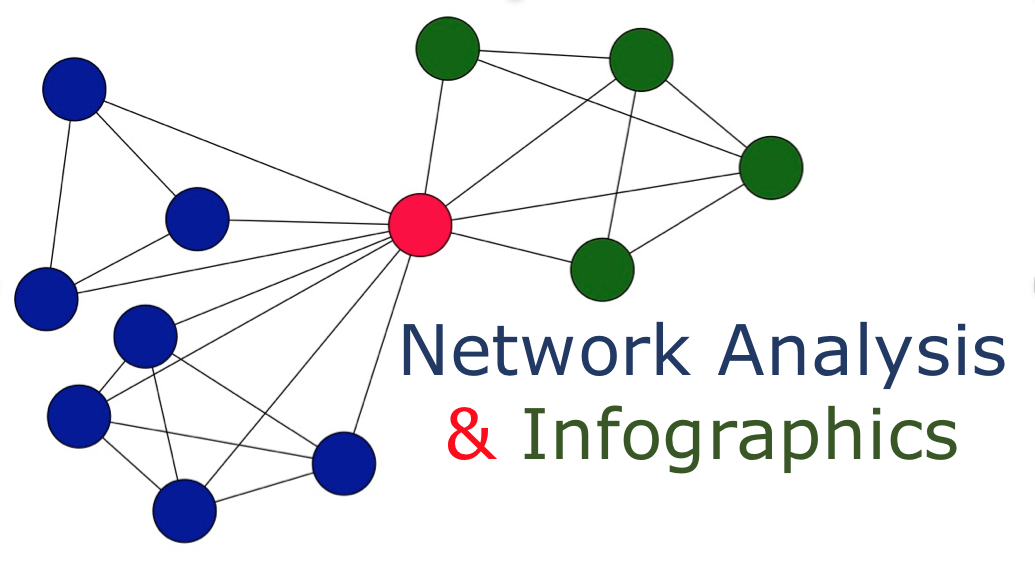
\includegraphics[width=2.5cm]{../_shared_pics/logo}

\medskip

\textit{{\color{dkgreen}{Week 8: 18 March 2022}}}\\
}


\date{} % Date, can be changed to a custom date

\begin{document}

\begin{frame}
\titlepage % Print the title page as the first slide

\begin{textblock*}{10pt}(0pt, 0.9\textheight)

\includegraphics[width=4cm]{../_shared_pics/SPRU.png}
\end{textblock*}

\end{frame}



%=======================================================
%	Learning outcomes
%=======================================================


\begin{frame}
\frametitle{\insertsection}
\framesubtitle{Learning Outcomes}

\centering
\begin{tabular}{lp{5.5cm}l}
\toprule
\multicolumn{2}{l}{\textbf{Learning outcome}} & \textbf{Assessment mode}\\
\hline
\\
1 & 
Explain the concept of network and list the main network indicators & 
ESS\\
\\
\rowcolor{green!20}2 &  
Describe and apply the major techniques for the collection of network data and their statistical analysis & 
ESS, GPN + GWS\\
\\
3 & 
Identify the main characteristics of networks by means of network measures  & 
ESS, GPN + GWS\\
\\
4 &
Employ network analysis techniques to produce network data-based infographics & 
GPN + GWS\\
\\
\bottomrule
\multicolumn{3}{l}{\scriptsize Note: ESS: Essay; GPN: Group Presentation; GWS: Group Written Submission}\\
\end{tabular}

\end{frame}

%------------------------------------------------



%=======================================================
%	Intro slides
%=======================================================

\begin{frame}
\frametitle{Overview}
\tableofcontents[hideallsubsections]
\end{frame}




%=======================================================
% Modelling and inference of networks [recap]
%=======================================================
\section{Modelling and inference of networks [recap]}
%------------------------------------------------

\bgroup
\setbeamercolor{background canvas}{bg = navyblue}
\begin{frame}[plain]{}
\begin{center}
\color{white}{\Huge\insertsection}
\end{center}
\end{frame}
\egroup

%------------------------------------------------


\begin{frame}
\frametitle{\insertsection}


    \begin{itemize}
    
    \item {\color{blue}{Mathematical models}}\\
    Based on `simple' probabilist rules to capture specific mechanisms
        	
    	\begin{itemize}
		\item  {\color{blue}{Random graph models}} assume $\mathbb{P}_{\theta}(G)$ to be a uniform distribution
			\begin{itemize}
			\item {\color{blue}{Erd\'os-R\'enyi}} random graph model
			\item {\color{blue}{Bernoulli}} random graph model
			\item {\color{blue}{Generalised}} random graph models
			\end{itemize}

		\item  {\color{blue}{Models based on mechanisms}} mimic certain properties observed in the real world
			\begin{itemize}
			\item {\color{blue}{Small-worlds}} models
			\item {\color{blue}{Preferential attachment}} models
			\end{itemize}
		\end{itemize}

\medskip

    \item {\color{blue}{Statistical models}}\\ 
     The observed network is considered as one of the possible realisation of a process
    
    	\begin{itemize}
		\item {\color{blue}{Exponential Random Graph Models (ERGM)}}: the {\color{blue}{presence/absence of a tie}} is the response variable that is dependent on {\color{blue}{endogenous}} and {\color{blue}{exogenous}} factors


		\item{\color{blue}{Stochastic Actor-Oriented Models (SAOM)}}: The co-evolution of a network structure and attributes is modelled as a stochastic process 

		\item {\color{blue}{Network Block Models}} model the propensity to establish a tie between two nodes as dependent on the `class' membership of the two nodes    	\end{itemize}

	\end{itemize}
	
\end{frame}



%=======================================================
% Modelling and inference of networks in igraph
%=======================================================
\section{Modelling and inference of networks in \textit{igraph}}

%------------------------------------------------

\bgroup
\setbeamercolor{background canvas}{bg = navyblue}
\begin{frame}[plain]{}
\begin{center}
\color{white}{\Huge\insertsection}
\end{center}
\end{frame}
\egroup

%------------------------------------------------

\begin{frame}
\frametitle{\insertsection}

\centering
\footnotesize
\begin{tabular}{ll}
\toprule
\textbf{Model} & \textbf{igraph function}\\
\hline
\\
\textbf{Mathematical models}\\
Erd\'os-R\'enyi 							& erdos.renyi.game()\\
Bernoulli									& erdos.renyi.game()\\
Generalised									& degree.sequence.game()\\
Small-worlds			    				& sample\_smallworld()\\
Preferential attachment 					& sample\_pa()\\
\\
\textbf{Statistical models} (not in this module)\\
Exponential Random Graph Models (ERGM)  		& `ermg' package\\
Stochastic Actor-Oriented Models (SAOM) 		& `RSiena' package\\
Network Block Models						& `blockmodels' package\\
\\
\bottomrule
\end{tabular}

\end{frame}

%-----------------------------------------------





%%=======================================================
%	Next time ...
%%=======================================================
\section*{Next time ...}
%------------------------------------------------

\bgroup
\setbeamercolor{background canvas}{bg = navyblue}
\begin{frame}[plain]{}
\begin{center}
\color{white}{\Huge\insertsection}
\end{center}
\end{frame}
\egroup

%------------------------------------------------

\begin{frame}
\frametitle{\insertsection}

\begin{itemize}

\item 	\textbf{Lecture: Innovation networks}
	\begin{itemize}
	\item Use of network analysis to map science and technology
	\end{itemize}	
	

\medskip
\medskip

\item 	\textbf{Seminar: Innovation networks}
	\begin{itemize}
	\item Practice with VOSViewer
	\end{itemize}

		
\end{itemize}

\end{frame}

%------------------------------------------------




\end{document}